In this part of the report, results of the PyTorch experimentation are described, as well as a quick hint to the differnece between ELU and TanH.

\subsection{Experimental design: Getting the MLP to 0.52 and beyond}
In the experiment, the goal was to get the MLP to 0.52 accuracy. To do this, a number of test-cases were considered. To prevent an 
explosion of the parameter space (and learn to understand simple changes better for the scope of this project),
changes were alternated most of the time, rather than combining them together. In the following table, the results of various experiments.
To ensure an easy overview, all the cells that contain a "-" use the default parameters as provided in the original code.

Furthermore, for batchnorm, an 'X' indicates that it has been used. The batchnorm was utilized only on hidden layers,
and not on the output layer.

The best performing is the bottom row in the following table:

\begin{table}[h]
    \begin{tabular}{@{}lllllll@{}}
    \toprule
    optimizer & hidden\_layers & batchnorm & batch-size & act\_fn & max\_steps & results \\ \midrule
    -         & -              & -         & -          & -       & -          & 0.451   \\
    adam      & -              & -         & -          & -       & -          & 0.461   \\
    -         & -              & -         & 64         & -       & -          & 0.41    \\
    -         & -              & -         & 256        & -       & -          & 0.456   \\
    -         & -              & X         & -          & -       & -          & 0.412   \\
    -         & -              & -         & -          & -       & 10000      & 0.480   \\
    -         & -              & -         & -          & tanh    & -          & 0.353   \\
    -         & 64,128         & -         & -          & -       & -          & 0.426   \\
    adam      & 64,128         & -         & -          & -       & -          & 0.421   \\
    adam      & 64,128         & -         & -          & -       & 10000      & 0.462   \\
    adam      & 64, 128        & X         & -          & -       & 10000      & 0.524   \\
    adam      & 64,128,256     & X         & -          & -       & 10000      & \textbf{0.531}   \\ \bottomrule
    \end{tabular}
    \caption{Runs with various permutations}
\end{table}

\begin{figure}%
    \centering
    \subfloat[\centering Training loss for default settings]{{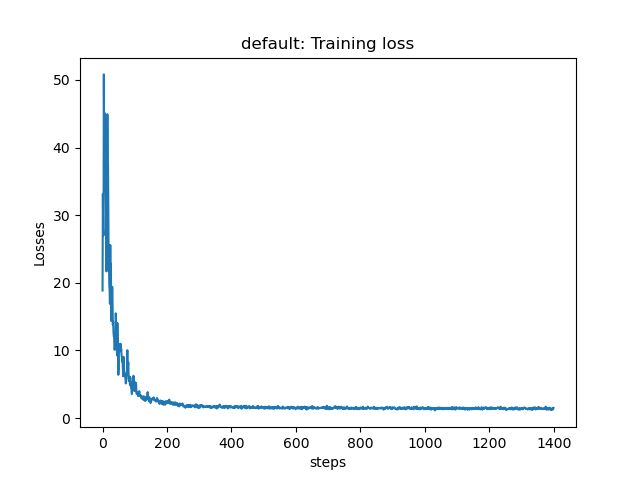
\includegraphics[width=6.5cm]{images/pytorch-mlp-default.train_loss.png} }}%
    \qquad
    \subfloat[\centering Test accuracy for default settings]{{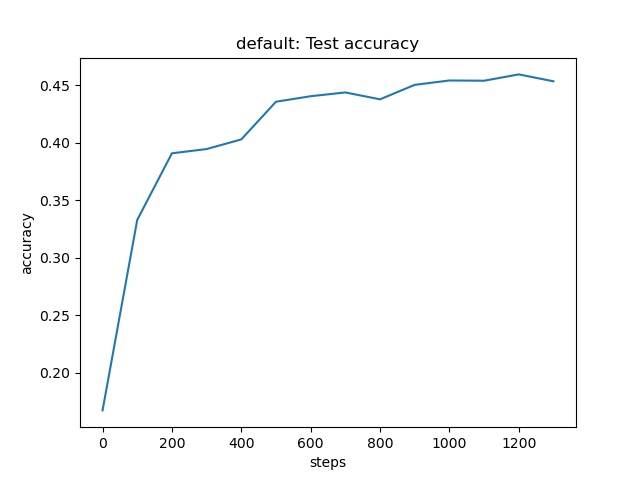
\includegraphics[width=6.5cm]{images/pytorch-mlp-default_test_accs.png} }}%
    \caption{Default performance, test and train}%
    \label{fig:defaults}%
\end{figure}

\begin{figure}%
    \centering
    \subfloat[\centering Training loss for best settings]{{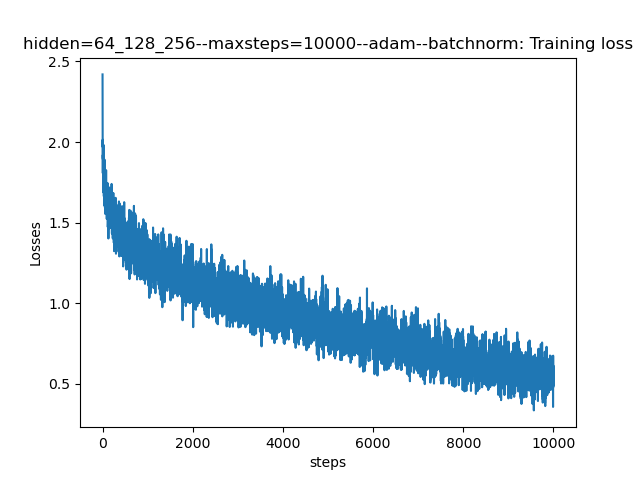
\includegraphics[width=6.5cm]{images/pytorch-mlp-hidden=64_128_256--maxsteps=10000--adam--batchnorm.train_loss.png} }}%
    \qquad
    \subfloat[\centering Test accuracy for best settings]{{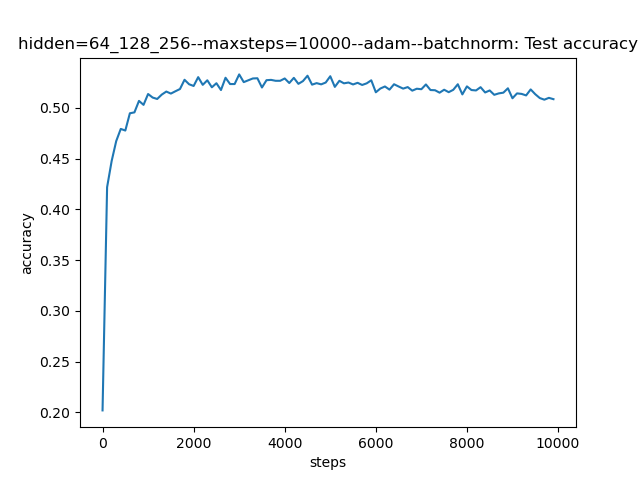
\includegraphics[width=6.5cm]{images/pytorch-mlp-hidden=64_128_256--maxsteps=10000--adam--batchnorm.test_accs.png} }}%
    \caption{Best performance, test and train}%
    \label{fig:defaults}%
\end{figure}

In the end, the best performance turned out to be the inclusion of batch-norm with more steps and more layers.
Important to note, was that especially when adding batch-norm, the ability to generalize with more layers started improving
tremendously.

\subsection{ELU vs TanH}
Some of the main benefits of using TanH, is that it provides a very clear bound for the activation values. 
ELU has no upper boundary, meaning that values could theroretically become huge, and rely on regularization
techniques. 

Drawbacks of Tanh relate to both slightly more expensive computation of the gradient of Tanh (more complex than
the very simple form of the ELU), and the dense layer weights it allows. With ELU, many insignificant weights
go to practically 0, whereas with Tanh, the weights are scaled somewhere between -1 and 1. Furthermore, 
networks with Tanh activation functions have converged a lot slower in this example for instance. 

Tanh could be used for outputting your values to a particular characteristic (e.g [-1, 1]). If the output
of your model requires this, Tanh can be used. ELU should never be used as output activation for your network.